\documentclass{article}

\usepackage[utf8]{inputenc}
\usepackage[T1]{fontenc}
\usepackage{graphicx}
\usepackage{listings}
\usepackage{color}
\usepackage{gb4n}
\usepackage{tipa}
\usepackage{lingsty}
\usepackage{ipashortcuts}
\usepackage{rotating}
\usepackage{times}
\usepackage{textcomp}
\usepackage{lingsty}

%-----
\usepackage[authoryear]{natbib}
\bibpunct[:]{(}{)}{,}{a}{}{,}
\setlength{\bibsep}{0.05cm}



\newcommand{\todo}[1]{\footnote{\textbf{todo:} #1}}
% \newcommand{\imgpath}{} 
\glossSTDmode
     

\title{The grammatical description as a collection of form-meaning-pairs}
\author{Sebastian Nordhoff} 

\newcommand{\imgpath}{./}
\begin{document}

\renewcommand\chapname{Grammars as form-meaning-pairs}	
\renewcommand\longchapname{The grammatical description as a collection of form-meaning-pairs}
\renewcommand\shortauthor{Sebastian Nordhoff}
\renewcommand\longauthor{Sebastian Nordhoff\\ Max Planck Institute for Evolutionary Anthropology}
\chapter*{\longchapname}
\chapterauthor{\longauthor}
\mytoc{} 
 
\begin{abstract}
This paper analyzes the structure of books containing grammatical descriptions and builds up on work by \citet{Good2004}. It argues that the discussion of morphology, syntax, semantics, and intonation found in grammatical descriptions can be seen as a collection of interdependent form-meaning-pairs. These form-meaning-pairs form part of the larger structure of frontmatter, mainmatter and backmatter \citep{Mosel2006craft} and have themselves an internal structure which includes, among other things, linguistic examples as formalized by \citet{BowEtAl2003}.
\end{abstract} 

\section{Introduction}
In this paper I will be concerned with the structure of a certain genre of texts, namely grammatical descriptions.\footnote{I would like to thank Jeff Good, Nick Thieberger, and Michael Cysouw for comments on earlier versions of this paper.} These texts have as an aim to store knowledge about the grammatical structure of a language, which may have a long literary tradition like French, or about which little may be known, as for Vedda, a small language in Sri Lanka. One thing which is important in the context of this paper is that I am dealing with \em texts \em and not with abstract entities like computational grammars which generate sentences \citep{Maxwelltv}. Neither do I deal with the mental representations of grammatical knowledge. While I acknowledge the relevance of the latter two concepts, which form an interesting topic for formalization in themselves, in this paper I will concentrate on texts which are used to communicate grammatical information about a language from a knowledgeable person (the describer) to a person wishing to know more about the language (the reader). This is to say, I treat the  ``grammatical description as a communicative act'' \citep{Payne2006}.



% The text genre of descriptive grammar has evolved over time. One can distinguish at least the following `models' of grammar writing: missionary, Indo-Europeanist, American structuralist, tagmemics, and functional-typological.\footnote{As stated above, I will exclude more theoretical approaches to grammar. An example for such approaches is for instance the description of Kikuyu in the framework of Transformational Grammar by \citet{Overton1972}.}
% As for diversity within the kind of publication, one can distinguish full grammars, sketch grammars and short discussions of a certain topic. See \citet{Hammarstroem2007} for an overview.


\section{Content-based and form-based structures}
In an ideal world, all grammatical descriptions would conform to the same schema. Once this schema is established and applied to all grammars, the reader will be able to navigate a new description very easily. An approach pursuing the unification of the description of grammatical knowledge is for example the Crosslinguistic Reference Grammar project \citep{Peterson2002,Zaefferer2006,Blacktv}. This approach presents a more or less elaborate apparatus for filling in  grammatical information in predefined fields. The value of these approaches is heavily  dependent on the quality of the underlying apparatus. In case the language in question does not exhibit a required phenomenon,\footnote{For 
 a non-technical overview of how little we can assume about language structure, see \citet{EvansEtAl2009BBS}.
} 
or it shows phenomena which were not known at the time when the apparatus was designed, the description cannot be implemented. Keeping track with theoretical developments (Upward-compatibility) seems to be a reasonable expectation for a formalization of grammatical description,\footnote{See 
 \citet{Mosel2006craft} for the necessity to update theoretical analyses.
} 
but it is unclear how this can be done with a rigid formalization of `what grammar is like' at the foundation of the apparatus.  Furthermore, an apparatus based on the predefined categories necessarily relies on the cross-linguistic applicability of these categories, but it is still subject to debate whether it is even possible to formulate crosslinguistically valid categories at all \citep{Haspelmath2007LT}. Moreover, language describers who do field work in remote places often have a strong personality with a disliking for being told how to describe `their' language. The feeling that `their' language is unique and cannot be pressed into a one-size-fits-all approach is widespread \citep{Weber2006grow}. Even without the fundamental problems alluded to above, it is unclear whether a `universal schema' is actually in line with the wishes of the describers. Finally, a universal schema is difficult to retrofit on already existing descriptions, which might be desirable if one wants to broaden the domain of semantic searches.

The `universalist' or content-based schemas mentioned above have as an implicit aim to structure what grammar is like, with `grammar' being used in its sense of `mental representation'. Following \citet{Good2004} and \citet{Nordhoff2008jldc}, I take a slightly different approach in structuring what \em grammatical descriptions \em are like. This approach can be called `form-based'. In the content-based approach, the elements of the structure are phonemes, words,  suffixes etc, while the form-based approach has paragraphs, examples,  and glosses as its elements. No claim is made about the universal applicability of the grammatical terms in the descriptions. Every author can describe the language how they see fit. However, the hypothesis is that grammar authors will make use of a number of typical textual elements like `linguistic examples', `paradigm tables',  `word-gloss-pairs' etc \citep{Good2004}. \citet{Good2004} surveys a sample of grammars and lists recurring structural elements, which are nested in a certain way. The highest structural element he recognizes is the `annotation', which can contain `exemplars', `prose', `references' and `links to ontologies', and further annotations in a recursive fashion. He formalizes this nested structure in a DTD. The linguistic example itself is at a lower level in the structure. Theoretical discussions of its structure can be found in \citet{Drude2002},   formalizations are given in \citet{Peterson2002} or \citet{BowEtAl2003}. In this paper, I want to concentrate on the higher elements in the structure, i.e. chapters and sections, while also refining Good's analysis of the `annotation'. I use lower level elements occasionally where necessary, but often omit them to keep the presentation visually appealing and free of clutter. My basic approach has as an aim to be compatible with \citet{BowEtAl2003} on the low level and \citet{Good2004} on the mid-level.

\section{The sample}


I will exemplify my claims in this paper by a sample of descriptive grammars which includes all traditions and publication forms and covers different areas of the globe. The sample consists of

\begin{itemize}
 \item \citet{Bloomfield1962}, a grammar of the North American language Menomini
 \item \citet{Seiler1985}, a grammar of the North American language Cahuilla *
 \item \citet{LiEtAl1981}, a grammar of Mandarin Chinese
 \item \citet{Epps2008}, a grammar of the Amazonian language Hup
 \item \citet{Buechel1939}, a grammar of the North American language Lakota *
 \item \citet{Haspelmath1993}, a grammar of the Caucasian language Lezgian * 
 \item \citet{Frohnmeyer1889}, a grammar of the Indian language Malayalam
 \item \citet{Newman2000}, a grammar of the Subsaharan language Hausa *
\end{itemize}

While all books were consulted, a general discussion will take up too much space, which is why the general findings are discussed based only on the starred items in the list above. In the remainder of this paper, I will follow \citet{Good2004} in  claiming that grammatical descriptions are semi-structured texts. When they are annotated for structure, semantic searches become possible, which is a useful resource for typologists. Figure \ref{fig:lezgian} from \citet{Haspelmath1993} illustrates a typical layout of a descriptive grammar.


\begin{figure}
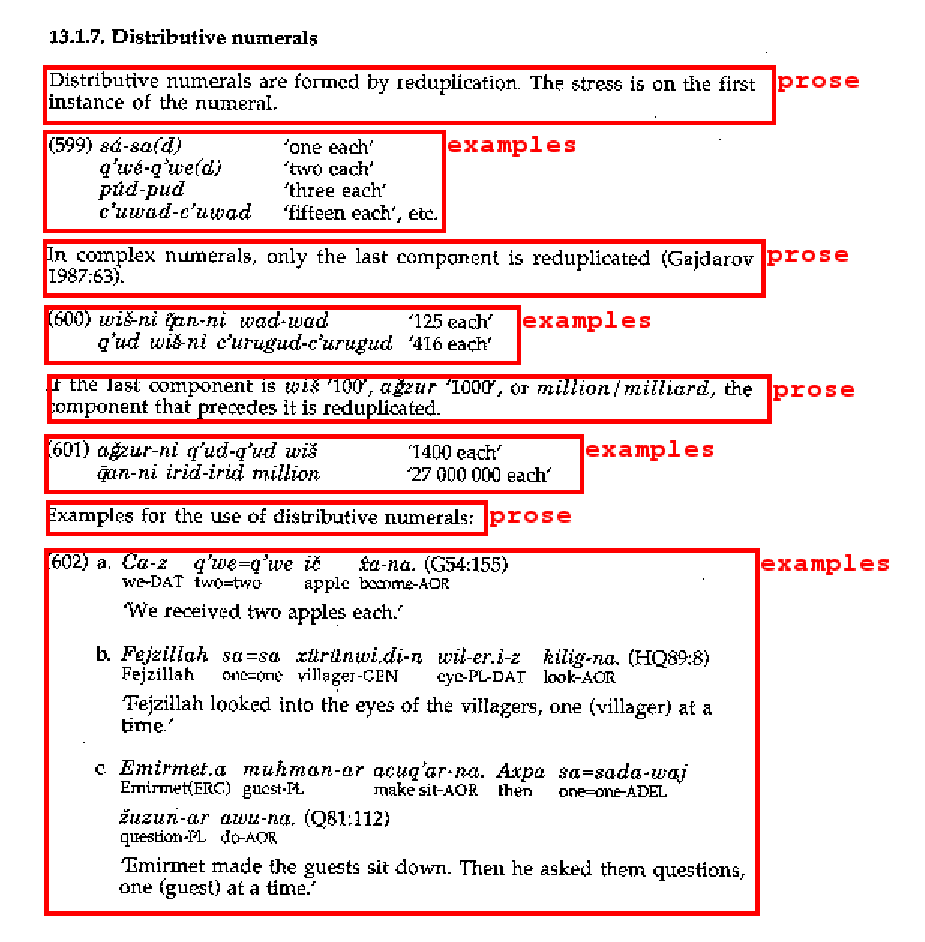
\includegraphics[width=\textwidth]{\imgpath/lezgian} 
\caption{The discussion of the distributive numerals in \citet{Haspelmath1993}}
\label{fig:lezgian}
\end{figure}


In Figure \ref{fig:lezgian}, the discussion is made up of prose, which is found before and after examples in a particular format which are use to illustrate the topic at hand, distributive numerals in this case. As a first step in structuring the text, we can separate the examples from the prose which discusses them \citep[cf.][]{Good2004}. The internal structure of the examples can then be worked out, as done for instance in \citet{BowEtAl2003}. The prose part has received less attention overall, which is why I will focus on this aspect here, next to the whole overarching structure of the book.

% In order to appreciate the internal diversity of the genre, a short historical overview is needed.
% The first major current of grammatical description of lesser known languages was missionary linguistics. In order to preach to the heathens, one had to know their language. So practical grammars of these languages were produced by missionaries to be handed over to new missionaries. The academic interest in the study of foreign language rose with American Structuralism in the beginning of the 20th century. Boas, Sapir and Bloomfield took on the task to describe the native American languages. It was in this period that the idea of describing a language in its own terms gained popularity. This contrasts with the missionary grammars, which often followed a model based on Latin or Greek grammar.


\section{The structure of grammatical descriptions: an overview}
Taking a look at the table of contents of the books in the sample, we find a certain recurrent ordering in the topics discussed. I take these findings to be uncontroversial, so I give an abbreviated XML-notation right away.\footnote{The 
 actual ordering of the chapters in the mainmatter may differ \citep{Mosel2006craft}, but what it is important here is that they are discussed as part of the mainmatter; the actual internal ordering is less relevant, as will be discussed below.
}

\ea\label{xml:book:intro}
\begin{verbatim}
<book>
  <frontmatter>
    <tableofcontents/ >
    <listoftables/ >
    <listoffigures/ >
    <listofabbreviations/ >
    <acknowledgments> ...  </acknowledgments>
 </frontmatter>
  <mainmatter>
    <background> ... </background>
    <phonology> ... </phonology>
    <morphology> ... </morphology>
    <syntax> ... </syntax>
    <semantics> ... </semantics>
 </mainmatter>
 <backmatter>
  <references/>
  <wordlist/>
  <texts>
    <text id="story1"> ... </text>
    <text id="recipe3"> ... </text>
  </texts>
 </backmatter>
</book>
\end{verbatim}
\z

The nature, relevance and functions of front- and backmatter are similar to what we find in other kinds of scientific books \citep{Mosel2006craft} so that the need to discuss these parts in this paper is less urgent. I will focus on the parts of the mainmatter then.
% Sperberg-McQueen and Bernard 2002 on TEI of dictionary

\section{The structure of the mainnmatter}
\subsection{Background}
Grammatical descriptions typically contain a chapter on the sociohistorical background of the language \citep{Lehmann2002}. In that chapter, the history and current sociological and political situation of the speech community is discussed. Topics covered are genealogical affiliation, geographical and political distribution, demographic factors such as ethnicity, religion, occupation and institutional representation. This part of the mainmatter does not seem to exhibit particular strong recurring structure and it does not seem wise to impose too tight a skeleton on it, so that I will treat it as unstructured data here.

\subsection{Morphosyntax: form-meaning-pairs ordered according to form}
Departing from the order normally found of books, I will now first discuss morphosyntax before coming back to phonology -- which is normally the first thing to be discussed -- in a minute. Depending on the language at hand, the division between morphology and syntax can be clear or rather subtle. While in Latin, the distinction is easy in most cases, other languages, like Tamil for instance, present challenges to the analyzer when they have to decide whether a given item is a suffix, an enclitic or an independent particle. There are ongoing theoretical discussions in particular languages about whether there is a division between morphology and syntax, and where it would be located (See \citet{CulicoverEtAl2005} for an overview for the English facts, \citet{Lehmann2002} for the consequences for language description). In light of these facts, it does not seem wise to impose a division in the schema until the differences are sorted out. What morphological and syntactical analyses have in common is that there is a certain form X which is said to have a certain function F. Whether X is treated as belonging to the morphological domain or to the syntactic domain is not substantial here. As an example, we can take the English possessive marker \em 's\em. No matter the analysis, we can say that \em 's \em is used to encode possession, widely construed. This is to say we are dealing with a \em form-meaning-pair\em.  The form \em 's \em of the English language is paired with the meaning \em possession\em. In this paper,  I propose that most of the morphosyntax of a language can be treated as discussion of form-meaning-pairs (henceforth abbreviated as `fomp').\footnote{A 
 `fomp' is a subset of the `Annotation' element proposed by \citet{Good2004}. `Annotations' are broader and could be used for other domains as well. It is a topic for further research to determine the relations between the general superordinate `annotation' type and the subset of form-meaning-pairs on the one hand and other types of description used in grammars (e.g. phonology)  on the other hand.
} 
Form-meaning-pairs consist of a topic of the discussion, which is at the same time the lemma (the name if you want) of the discussion. This topic is discussed with the help of illustrative examples\footnote{It
 seems sensible to have a container to contain a collection of individual examples illustrating aspects of the same phenomenon each. \citet{Good2004} calls this container \texttt{$<$exSet$>$}. In line with the general use of full words in markup in this paper, I use \texttt{$<$examples$>$}, but the two terms can be subsituted for each other.
} 
and surrounding prose.\footnote{The
 prose has an internal structure as well, consisting of running text interspersed with some special elements like references, \trs{word}{gloss}-pairs, technical terms and references. Specialized markup for these elements and links to ontologies enhance the computational usability of the grammatical description \citep{FarrarEtAl2003,Good2004}. For reasons of space and in order not to clutter the examples with tags, I omit the markup around the mentioned elements.
} 
We can illustrate this with the following fragment:

\ea
\label{xml:fofomp:intro}
\begin{verbatim}
<fomp type="form-to-function" lemma="'s">
  <prose>
    The phrasal affix <form> 's" </form>  is used to
    code <meaning> possession </meaning>.
  </prose>
  <examples>
    <example> My friend's car </example>
  </examples>
   <prose>
     As we see in the example above, the affix
     attaches to the right edge of an NP, in this
     case <objectlanguage> My friend </objectlanguage>.
   </prose>
</fomp>
\end{verbatim}
\z
 

As a consequence of the bipartite nature of the form-meaning-pair, discussion of the sign can focus on the form part (signifiant) or on the meaning part (signifié) \citep{Lehmann2004funkt}. Figure \ref{fig:cahuilla} from \citet{Seiler1985} shows a neat separation between the discussion of formal properties and the discussion of functional uses. In the formal part on top, marked in red, allomorphs, a purely formal phenomenon, are discussed, while in the functional part on the bottom, marked in blue, the communicative situations where this morpheme can be used are explicated, in this case \textsc{wishes}.

\begin{figure}
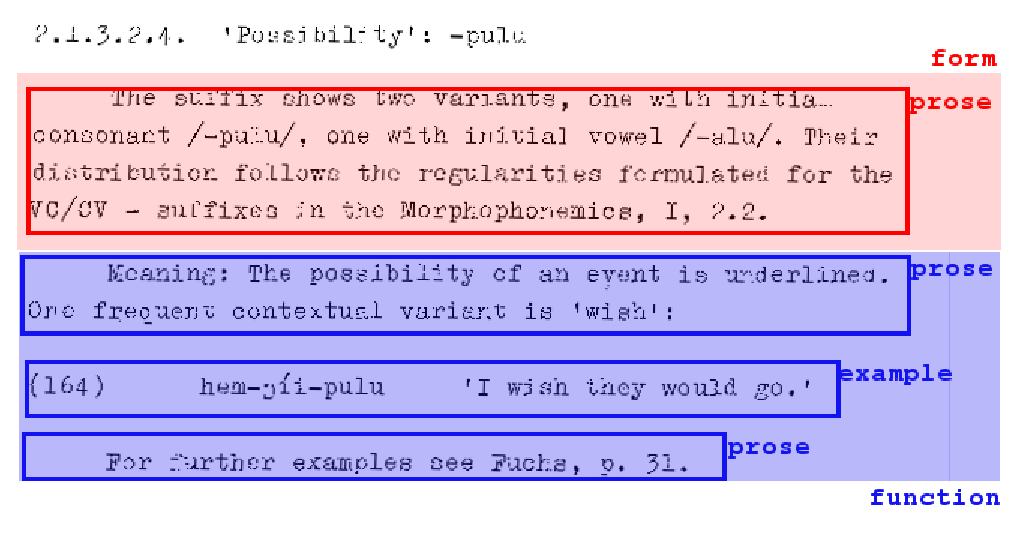
\includegraphics[width=\textwidth]{\imgpath/cahuilla} 
\caption{The discussion of the morpheme \em pulu- \em in \citet{Seiler1985}}
\label{fig:cahuilla}
\end{figure}


The division in a discussion of formal properties and functional properties can be squared with the alternation between prose and examples. Figure \ref{fig:hausa:ma} shows such a more complex configuration.

\begin{figure}
\includegraphics[height=\textheight]{\imgpath/hausa-agentma}
% hausa-agentma.png: 0x0 pixel, 0dpi, 0.00x0.00 cm, bb=
\caption{The discussion of the agentive morpheme \em ma- \em in \citet{Newman2000} shows a division of formal and functional properties, and a further subdivision in
\\
 prose parts and example parts.}
\label{fig:hausa:ma}
\end{figure}

This structure of the text can be represented in semantic markup \xref{xml:fofomp:functionalformal}.

\ea\label{xml:fofomp:functionalformal}
\begin{verbatim}
<fomp>
  <formaldescription>
    <prose>
      <form> XYX </form> has the following properties
    </prose>
    <examples>
      <example> ...</example>
    </examples>
  </formaldescription
  <functionaldescription>
    <prose>
      <form> XYX </form> is used for <meaning> Function
      FGH </meaning>
    </prose>
    <examples>
      <example> ...</example>
    </examples>
  </functionaldescription>
</fomp>
\end{verbatim}
\z


The kind of discussions we find in morphology have similarities to what we find in lexicography \citep{SchultzeBerndt1998,Mosel2006craft,Weber2006grow}. First the forms are enumerated, then the possible meanings are given; additional information about domain, register or etymology may also be provided. In light of the similarity to the lexicon, I will follow a suggestion by \citet{LehmannEtAl2004} and call the space where these things are discussed \em Morphemicon\em.

\subsection{Collections of fomps}
In grammtical descriptions, as in other books, related phenomena are often grouped together. Sentences which cover related ideas are grouped into a paragraph, related paragraphs into sections, and related sections into chapters, with possibly some intervening levels \citep{Good2004}. The conceptual unity of a discussion within a grammatical description is typically reflected in typography by white space. Tight coherence is mirrored by little space (e.g. between sentences), while more loose coherence is expressed by blank lines between paragraphs or blank pages between chapters. These organizational blocks thus reflect the semantic structure of the grammatical description. In a book, they are necessarily ordered linearly. However, when discussing the members of a set of morphemes, there is no inherent order. To take the French question words
\trs{qui}{who},
\trs{quand}{when},
\trs{quoi}{what},
\trs{comment}{how},
\trs{où}{where},
\trs{pourquoi}{why}, no clear order of discussion suggests itself. The discussion of \em qui \em is pretty much independent of the discussion of \em quand\em, and both are independent of the discussion of \em où\em. The gist of the description does not change if you discuss \em qui \em before \em quoi \em or the other way round. The fact that in grammatical descriptions they are found in the sections numbered X.1, X.2, X.3 etc is simply a reflex of the requirement of the linear structure for printing. These numberings correctly indicate the subordination of these concepts to a higher complex of `question words' (X in the example above), but they incorrectly suggest an inherent  order among these items.\footnote{\citet{Good2004} 
 concurs with the non-linear structure but remarks that the logical independence of these sections may be forfeited for a gain in didactic usefulness. To remain within the French example, the discussion of \em quoi \em should probably take place before \em pourquoi \em because the former is a component of the latter.
} 
When creating the semantic markup for grammatical descriptions, we should not be fooled by incidental side effects of printing. However, the hierarchical structure of grammatical descriptions must be recognized. Some phenomena need to be discussed at an abstract level.

To take an analogy from classical zoologic taxonomy, in the family of \em Felinae \em  we find the genera \em Lynx, Leopardus, Puma, \em and \em Felis\em, among others. There is surely no inherent order in discussing these genera, but some characteristics are shared among all members, e.g quadripedal, carnivore diet or moustaches. It would be redundant to state these facts at every individual level. They can better be discussed at the superordinate level of \em genus proximum\em. The same is true of linguistics. A semantic markup of grammatical description must provide for the possibility to state generalizations and sub/superordination. This is not a trivial problem. Here I would like to propose that this can be done by a general description followed by an enumeration of the members of the class with links to more detailed descriptions of the particular members. The XML-structure would be as follows:\footnote{For 
 reasons of simplicity, I omit the representation of `illustrative examples/paradigms' which are sometimes used in overview sections \citep{Good2004}.
}

\ea\label{xml:formlist}
\begin{verbatim}
<fomp type="formlist" name="Question words">
  <overview>
      <prose>
          Question normally start with the string "Wh".
          An exception is <form> how </form>. They are
          used to express <meaning> requests for
          information </meaning>. Question words normally
          trigger <form> do-support </form>.
      </prose>
  </overview>
  <ul>
    <li><form> Who </form></li>
    <li><form> What </form></li>
    <li><form> When </form></li>
    <li><form> Why </form></li>
    <li><form> Where </form></li>
    <li><form> How </form></li>
  </ul>
</fomp>
\end{verbatim}
\z

This list structure can be recursive \citep{Good2004}, so that deeper levels of subordination can be represented (free words$>$Nouns$>$Common Nouns$>$Count Nouns). Furthermore, multiple inheritance would also be possible.

As far as the treatment of formal (or semasiological) aspects is concerned, we thus have to distinguish two types of \textit{fomps}: a kind of  terminal node of the type ``form-to-function'' and a superordinate node of the type ``formlist''. The latter can include links to instances of the former.

The structure of the morphemicon can then be represented as in \xref{xml:morphemicon}. Note that the linear order of the elements is a coincidence here. The morphemicon is an \em un\em ordered list, as discussed above.\footnote{As
  an illustration of the unordered nature of fomps, we can take \citet{Newman2000}, who lists them in alphabetical order, the following is an excerpt from the table of contents:
  \begin{itemize}
  \item Prepositions
  \item Pro-Verb \em yi\em
  \item Pronouns
  \item Questions
  \item Reason and Purpose
  \item Reduplication
  \end{itemize}
}	

\ea\label{xml:morphemicon}
\begin{verbatim}
<morphemicon>
  <fomp type="formlist" name="Question words">
  ...
  </fomp>
  <fomp type="form-to-function" name="who">
  ...
  </fomp>
  <fomp type="form-to-function" name="what">
  ...
  </fomp>
  <fomp type="form-to-function" name="where">
  ...
  </fomp>
  <fomp type="form-to-function" name="why">
  ...
  </fomp>
  ...
  ...
  <fomp type="formlist" name="Demonstratives">
  ...
  </fomp>
  <fomp type="form-to-function" name="this">
  ...
  </fomp>
  <fomp type="form-to-function" name="that">
  ...
  </fomp>
</morphemicon>
\end{verbatim}
\z


\subsection{The treatment of examples: Bow, Hughes and Bird}

Besides the structure of the higher level elements and descriptive prose, the linguistic example is obviously central to the discussion of semantic markup. This area has received a seizable amount of research \citep{Drude2002,Peterson2002,BowEtAl2003}, which cannot be fully reviewed here. For the purposes of this paper, I adopt the XML-schema proposed by \citet{BowEtAl2003}, given for reference below.

\ea\label{xml:bbh}
\begin{verbatim}
<interlinear-text>
  <item type="title"> The Title</item>
  <phrases>
    <phrase>
      <item type="gls"> A phrasal translation</item>
      <words>
        <word>
          <item type="txt"> Word</item>
          <morphemes>
            <morph>
              <item type="txt"> Morph</item>
              <item type="gls"> Gloss</item>
            </morph>
            <morph>
              <item type="txt"> Morph</item>
              <item type="gls"> Gloss</item>
            </morph>
          </morphemes>
        </word>
      </words>
    <phrase>
  </phrases>
</interlinear-text>
\end{verbatim}
\z

This `raw' example can be further enhanced by information on meta-data (source, links to media files) and additional didactic annotations \citep[constituency, highlighting of important aspects][]{Good2004}.


\subsection{Extending formal description: beyond the morpheme}
In the paragraphs above I have discussed how morphemes can be linked to functions. However, morphemes are not the only meaning-bearing units in language. There are also constructions like \em VERB the TIME away \em e.g. \em dance/waltz/chat the night/evening away \em or more concrete \em kick the bucket \em \citep{CulicoverEtAl2005}. The particular meaning of these constructions is more than what is present in their morphemic parts, so that we must assume some meaning stemming from the construction itself \citep{FillmoreEtAl1993CxG,Goldberg1995CxG,Croft2001rcg}. Another example is the difference between \em John has come \em and \em Has John come?\em. In this case, the relative order of auxiliary and subject indicates whether we are dealing with an assertion or a question. The meaning-bearing units of a language are thus not exclusively atomic, but they can be complex as well \citep{Lehmann1993}. Furthermore, they are not always concrete as in the case of morphemes or idioms but they can also be schematic as in the case of the inversion questions. All this warrants the creation of a space where to discuss the meanings carried by these constructions. Following \citet{Goldberg1995CxG} I call this space \em constructicon\em.

The morphemicon deals with atomic and concrete elements, while the constructicon deals with schematic elements, which may be abstract or concrete. Both have in common that they deal with segmental material. Yet another complex bearing meaning in language is intonation, which is suprasegmental. The change of falling to rising intonation in the pair \em Jim's mother has come. \em vs. \em Jim's mother has come? \em has a predictable 	correspondence on the meaning side, the change of an assertion into a question. It seems best to treat intonation separated both from morphemes and constructions in a \em contouricon \em although there are of course some relations (WH-words trigger question intonation etc). The final structure of the morphosyntactic part is then

\ea\label{xml:semasiology}
\begin{verbatim} 
<forms>
 <morphemicon>
  <fomp type="morpheme" lemma="XX"> ... </fomp>
  <fomp type="morpheme"  lemma="YY"> ... </fomp>
  ...
 </morphemicon>
 <constructicon>
  <fomp type="construction" lemma="A B-C"> ... </fomp>
  <fomp type="construction" lemma="DE=F H G"> ... </fomp>
  ...
 </constructicon>
 <contouricon>
  <fomp type="intonation" lemma="HHL"> ... </fomp>
  <fomp type="intonation" lemma="HLH"> ... </fomp>
  ...
 </contouricon>
</forms>
\end{verbatim} 
\z

\subsection{Phonology}
The phonological part of grammatical description is normally structured as follows.

\ea\label{xml:phonology}
\begin{verbatim} 
<phonology>
  <segments>
    <phonemechart/ >
    <vowels> ... </vowels>
    <consonants> ... </consonants>
  </segments>
  <phonotactics> ... </phonotactics>
  <stress> ... </stress>
  <!-- <intonation> ... </intonation> -->
\end{verbatim}
\z

As discussed above, I propose to treat intonation as something which does not merely distinguish meaning (like phonemes) but which carries a meaning of its own, more like morphemes \citep[cf.][]{Mosel2006craft}.  Therefore, it can be meaningfully treated in the context of form-meaning-pairs, and there is no need to repeat the information in the phonological parts (although there should obviously be links between the two). This is why this element is commented out in \xref{xml:phonology}.

The remaining content in the phonological domain belongs to the domain of `distinguishing meaning'. This cannot be discussed in the context of form-meaning-pairs. The schmematization of this part will be left as a topic for future research.
 
\subsection{Semantics: form-meaning-pairs ordered according to function}
Above, I have discussed the structures we find in form-meaning-pairs based on morphemes and other forms.  This approach is called the form-to-function or semasiological approach. Let's call this perspective form-based form-meaning-pairs, or \em fo-fomps \em for short. It is possible to take the converse approach, i.e. function-to-form or onomasiological \citep{Gabelentz1891,Jespersen1924}. This approach is the one which is generally relevant in typological work, although it is less prevalent in extant grammatical descriptions \citep{Lehmann1980,
Comrie1998,
Lehmann1998,Lehmann2004funkt,
SchultzeBerndt1998,
Cristofaro2006,
Mosel2006craft,
Payne2006,
Zaefferer2006}, a notable example being \citep{Willett1991}. Figure \ref{fig:Willett} shows the table of contents of Willet's description of Southeastern Tepehuan

\begin{figure}

\begin{tabular}{ll}
  \begin{tabular}{ll}
  1 & Introduction\\
  2 & Phonology \\
  3 & Clause structure\\
  4 & Situations\\
  \hspace{.2cm}4.1 &Static situations \\
  \hspace{.2cm}4.2.& Dynamic situations \\
  5 & Entities\\
  6 & Settings\\
  \hspace{.2cm}6.1. & Location and direction\\
  \hspace{.2cm}6.2. & Time\\
  \hspace{.2cm}6.3. & Manner \\
  7 & Tense\\
\\
\\
\\
  \end{tabular}
  &
  \begin{tabular}{ll}
  8 & Aspect\\
  \hspace{.2cm}8.1 & Inception, termination and realization\\
  \hspace{.2cm}8.2 & Distinctiveness and simplicity \\
  \hspace{.2cm}8.3 & Resultative\\
  \hspace{.2cm}8.4 & Distribution, repetition and extent\\
  \hspace{.2cm}8.5 & Temporary and durative\\
  \hspace{.2cm}8.6 & Motion and transfer\\
  9 & Modality\\
  10 & Valence\\
  11 & Deixis\\
  12 & Specification\\
  13 & Coordination\\
  14 & Subordination\\
  15 & Continuity\\
  16 & Conclusion\\
  \end{tabular}
\end{tabular}
\caption{Excerpt from the table of contents of \citet{Willett1991}. For reasons of space, only selected subsections are shown.}
\label{fig:Willett}
\end{figure}


This is in many ways the mirror image of the former approach. Instead of taking a form and looking at the meanings it can express or the functions it can fulfill, we take a function and look at the forms it can be instantiated by. Let's call this perspective function-based form-meaning-pairs or \em fu-fomp\em. The division in prose parts and lists of examples is the same as above.

An illustrative example of the structure of a fu-fomp is given below in \xref{xml:fufomp:intro}. Note the similarity to example \xref{xml:fofomp:intro} above.

\ea\label{xml:fufomp:intro}
\begin{verbatim}
<fomp type="function-to-form" lemma="Comparison">
  <prose>
    The <function> comparative degree </function> of
    adjectives can be expressed by the suffix <form>
    -er </form> or by the particle <form> more </more>
  </prose>
  <examples>
    <example> Mary is taller than John </example>
    <example> Mary is more intelligent than
    John </example>
  </examples>
  <prose>
    As we see in the example above, short adjectives
    form the comparative with <objectlanguage>
    -er </objectlanguage> while longer adjectives take
    the particle <objectlanguage> more </objectlanguage>.
  </prose>
</fomp>
\end{verbatim}
\z




A more real-life example is given in Figure \ref{fig:lakota}, which shows the discussion of the function of comparison of adjectives in Lakota. This function can be instantiated by three different constructions. After an initial overview of what this section is about, three different constructions which can be used to convey this meaning are discussed. These are a) an adverb meaning `more', b) several other types of words with a rough meaning of `surpass' and finally c) a contrastive juxtaposition of the type `X is good and Y is bad'.

\begin{figure}
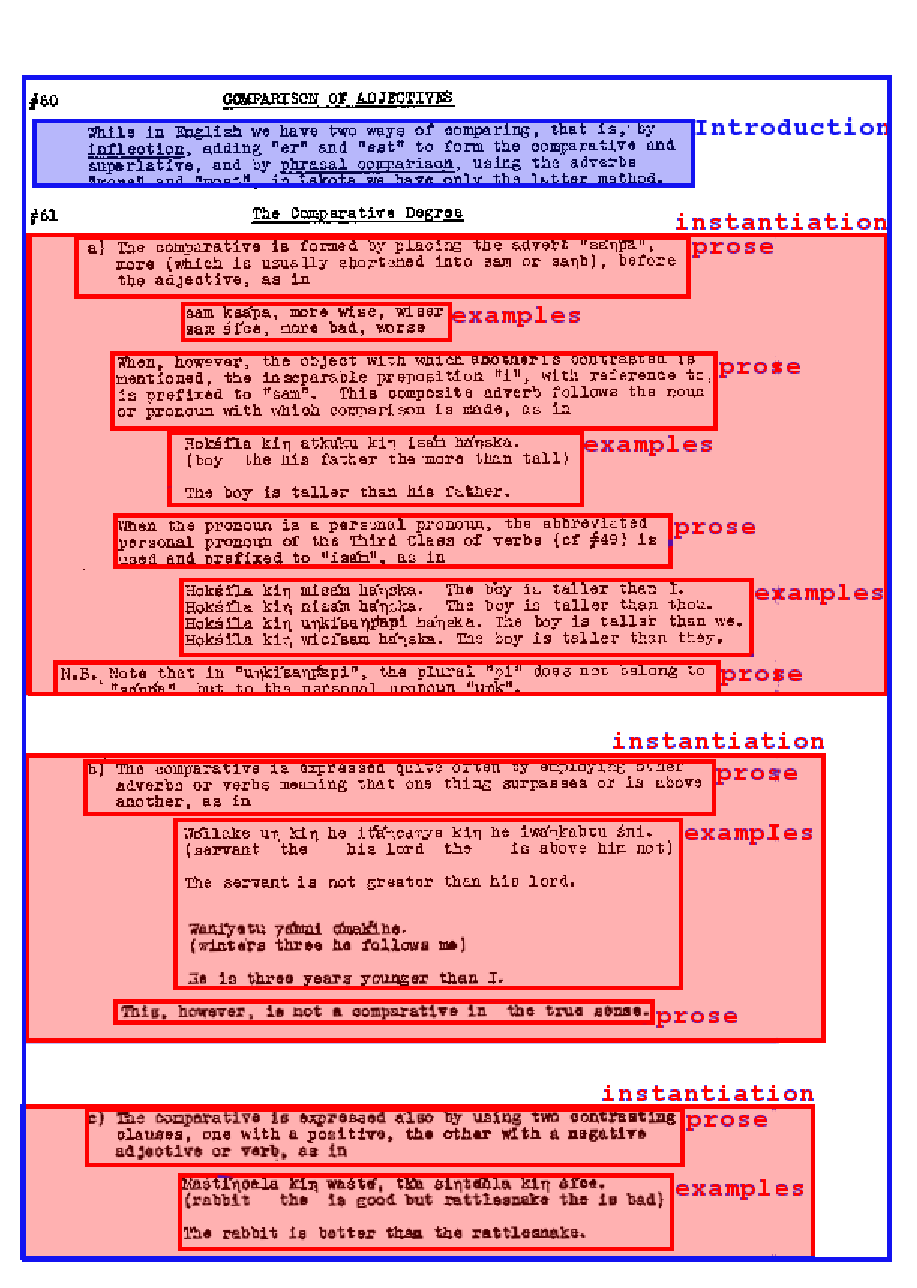
\includegraphics[height=\textheight]{\imgpath/lakota}
% lakota.png: 1179666x1179666 pixel, 0dpi, infxinf cm, bb=
\caption{The discussion of the function `Comparison of Adjectives' in Lakota in \citet{Buechel1939}, with three forms instantiating this function.}
\label{fig:lakota}
\end{figure}

Given that the readers of grammatical descriptions are normally expected to have a basic knowledge of the world, the introductory portions of fu-fomps tend to be short. There is no need to belabour the intended meaning of the function called `comparative degree' or `temporal reference prior to speech act' as this is pretty much self-evident from the naming. In some more involved domains involving less familiar concepts like e.g. the paucal, the introduction can be longer and illustrate the functional domain at hand in more detail. This is especially true for semantic distinctions presumed unfamiliar to the average reader, like alienability, evidentials, or the paucal mentioned above.

In a function-to-form approach, additional contrastive information can be provided about shades of meaning, frequency or register. This information is less commonly found in form-to-function approaches. Figure \ref{fig:tepehuan} from \citet{Willett1991} shows the description of a function and two formal instantiations thereof. Crucially, the two formal strategies come from different domains: the first one is a prefix (morphology) while the second one is a particle (syntax). In a form-to-function approach, the functional relatedness of these forms would have been difficult to convey. Furthermore, the two strategies can now be compared as to their felicity in different contexts, and their overall frequency. Without the functional \em tertium comparationis \em of `Intention' spelled out, this information would have been very difficult to find in the grammar.

\begin{sidewaysfigure}
 \centering
 \includegraphics[width=\textwidth]{\imgpath/tepehuan.png} 
 \caption{A function-to-form description of `Intention' in Tepehuan \citep{Willett1991}.}
 \label{fig:tepehuan}
\end{sidewaysfigure}



\subsection{Extending functional description}
I have shown above that different types of fo-fomps exist, namely those which belong to the morphemicon, the constructicon, and the contouricon. In what concerns fu-fomps, a similar division exists. We can distinguish meaning components which are purely semantic and relate to the communicated content. Examples are participants, events, space, and time as in \em John ate a cake at the party at midnight\em. These meaning components can be grouped in a \em semanticon\em. This purely semantic information is different from meaning components like topic and focus, which do not belong to the propositional content. An example would be the difference between \em John came \em and \em It was John who came\em. These sentences communicate the same semantic content and are truth-equivalent. Yet, there is a difference in information structure in that in the second sentence, the hearer is already expected to know that an act of coming occurred, which is not the case in the first sentence. These components of meaning which belong to information structure or discourse pragmatics can be discussed in a \em discoursicon\em. Speech acts are yet another type of function which is outside of both semantics proper and discourse. An example would be a request like \em Please do come, John\em. I will collect this interpersonal type of information in a \em pragmaticon\em. This division mirrors the layered structure of the clause as found in a number of contemporary grammatical theories like Role \& Reference Grammar  \citep{FoleyEtAl1984,VanValinEtAl1997rrg} or Functional Grammar \citep{Hengeveld1989,HengeveldEtAl2008fdg}. We can add this structure to the general outline of grammatical descriptions \xref{xml:fufofomp}.
\ea\label{xml:fufofomp}
\begin{verbatim} 
<forms>
 <morphemicon>
  <fomp type="morpheme" lemma="ab"> ... </fomp>
  <fomp type="morpheme"  lemma="def"> ... </fomp>
 </morphemicon>
 <constructicon>
  <fomp type="construction" lemma="A B-C"> ... </fomp>
  <fomp type="construction" lemma="DE=F H G"> ... </fomp>
 </constructicon>
 <contouricon>
  <fomp type="intonation" lemma="HHL"> ... </fomp>
  <fomp type="intonation" lemma="HLH"> ... </fomp>
 </contouricon>
</forms>
<functions>
 <semanticon>
  <fomp type="semantics" lemma="space"> ... </fomp>
  <fomp type="semantics"  lemma="kin"> ... </fomp>
 </semanticon>
 <discoursicon>
  <fomp type="discourse" lemma="argument focus"> ... </fomp>
  <fomp type="discourse" lemma="new topic"> ... </fomp>
 </discoursicon>
 <pragmaticon>
  <fomp type="pragmatics" lemma="requests"> ... </fomp>
  <fomp type="pragmatics" lemma="insults"> ... </fomp>
 </contouricon>
<pragmaticon>
\end{verbatim} 
\z

A more extensive subdivision into 13 subcategories of meaning can be found in \citet{Lehmann2004docu}.\footnote{Apprehension 
 and nomination, concept modification, quantification, reference, possession, space construction, predication, design of situations, temporal orientation, illocution and modality, contrasting, nexion, articulation of discourse
}  
These subcategories can be partitioned among the semanticon, discoursicon and pragmaticon, which will not be formalized here.


\subsection{Collections of fu-fomps}
Like fo-fomps in \xref{xml:formlist}, fu-fomps can also be arranged hierarchically, for instance the hierarchy

\ea Expressing time $>$ Expressing internal temporal structure $>$ Expressing imperfective aspect. \z

One can state general observations at the higher levels of the hierarchy ("Tense and aspect are nearly always expressed by prefixes") and more particular observations lower down in the hierarchy ("Progressive aspect can be expressed by \em papu- \em or by \em pipo-\em")

\ea\label{xml:funclist}
\begin{verbatim}
<fomp type="funclist" name="Expressing time">
  <overview>
      <prose>
          Expressions of time cover lexical solutions
          like <objectlanguage> aujourd'hui </objectlanguage>
          <gloss> today </gloss> or <objectlanguage>
          hier </objectlanguage> <gloss> yesterday </gloss>.
          When time is expressed by bound morphemes, these
          are normally <form> suffixes<form>. This is true
          for both tense and aspect.
      </prose>
  </overview>
  <ul>
    <li><meaning> Expressing tense  </meaning></li>
    <li><meaning> Expressing aspect </meaning></li>
  </ul>
</fomp>
\end{verbatim}
\z

What has been said above about collections of fo-fomps applies \em mutatis mutandis \em to collections of fu-fomps as well.


\subsection{Interaction of fo-fomp and fu-fomp}
\citet{Mosel2006craft} notes that an ideal grammatical description could actually be required to state everything twice: once from a formal perspective and again from a functional perspective. A recent grammar which does precisely that is \citet{Nordhoff2009phd}. The table of contents for the formal and the functional part are given in figure \ref{fig:nordhoff}.

\begin{figure}
\parbox[t]{6cm}{
 Verbs\\
 Nouns\\
 Adjectives\\
 Adverbs\\
 Copula\\
 Personal pronouns\\
 Interrogative pronouns\\
 Deictics\\
 Quantifiers\\
 Numerals\\
 Interjections\\
 Modal particles\\
 Negative particles\\
 Other particles\\
 Conjunctions\\
 Classifiers\\ 
 Affixes\\
 Simple clitics\\
 Bound words\\
 Nominal and verbal morphology\\
 Verbal predicates\\
 Existential predicate\\
 Modal predicate\\
 Nominal predicates\\
 Circumstantial predicate\\
 Adjectival predicate \\
 Noun phrases\\  
 Postpositional phrases\\
 Main clauses\\
 Relative clause\\
 Conjunctive participle clause\\
 Purposive clauses\\
 Subordinate interrogative clauses\\
 Supraordination\\
 The position of adjuncts\\
 Reported speech\\
 Agreement\\
}
\parbox[t]{6cm}{
Particpants\\
Participants of different entity orders \\
.\hspace{.5cm}Participant roles \\
% Mismatches between number of semantic roles and number of syntactic arguments \\
.\hspace{.5cm}Unknown participants \\
.\hspace{.5cm}Modifying participants \\
Predication\\
.\hspace{.5cm}States \\
.\hspace{.5cm}Events \\
.\hspace{.5cm}Causation \\
% Giving extra information beyond the nuclear predication\\
Modification\\
Space\\
.\hspace{.5cm}Figure-ground relations \\
.\hspace{.5cm}Indicating   spatial orientation  \\
Time\\
.\hspace{.5cm}Figure and ground \\
.\hspace{.5cm}Phasal information \\
.\hspace{.5cm}Aspectual structure \\
Quantification\\
% Quantification of referents \\
% Event quantification \\
% Temporal frequency \\
Modality\\
Conditionals\\
Gradation\\
% Equation \\
% Similarity \\
% Superiority \\
% Inferiority \\
% Superlative \\
% Elative \\
% Abundantive \\
% Caritive \\
% Correlative \\
Comparison\\
Possession\\
.\hspace{.5cm}Assertion of the possessee \\
.\hspace{.5cm}Possession of abstract concepts \\
.\hspace{.5cm}Assertion of the possessor \\
% Presupposition of the possessor and the possessee \\
Negation\\
Kin\\
Referents and reference\\
Topic\\
Presupposition and assertion\\
Canceling implicatures\\
Parsing\\
Speech acts\\
Blending in the social tissue\\
}
\caption{The formal (left) and functional (right) table of contents of Nordhoff's grammar of Upcountry Sri Lanka Malay.}
\label{fig:nordhoff}
\end{figure}
 
The diligent reader will have noticed that the fo-fomp in example \xref{xml:fofomp:intro} and the fu-fomp in example \xref{xml:fufomp:intro} contain some additional markup. This markup can be used to link the form-to-function (semasiological) description with the function-to-form (onomasiological) description, a common desideratum for electronic grammars \citep{Comrie1998,Lehmann1998,Zaefferer1998,Mosel2006craft,Nordhoff2008jldc}. I will illustrate this with a fragment of the grammar of French, namely question formation.

In French, there exist three principal ways to request information from the hearer:  rising intonation contour, a question formative \em est-ce que\em,\footnote{For 
 the ease of discussion, I essentially treat \em est-ce que \em as unanalyzable here. It is true that this introducer can be segmented into \trs{est}{is}, \trs{ce}{this} and \trs{que}{that}, but the construction has grammaticalized to such an extent that there is little awareness of the internal constituency. This can also be seen from the fact that an authortitative reference grammar of French \citep{GrevisseEtAl1995} treats this construction as basically monomorphemic. The term `introducer' (`introducteur') is also taken from this work.
} 
and inversion. These three patterns are illustrated in \xref{ex:frenchquestions}. \xref{ex:frenchquestions:assertion} gives the declarative sentence for comparison.

\ea\label{ex:frenchquestions:assertion}
\gll Elle danse.\\
     She dances\\
    `She dances/is dancing'
\z
 
\ea\label{ex:frenchquestions}
\ea $\widetilde{\rm Elle}$ $\stackrel{\_\diagup\hspace{.7cm}}{\rm danse}$?
% \ea Elle $\widetilde{\rm danse}$?
\ex Est-ce qu'elle danse?
\ex Danse-t-elle?\\
 `Does she dance/Is she dancing?'
\z
\z

We see that there is a many-to-one relation form form to function, and a one-to many relation from form to function. We can illustrate this as in Figure \ref{fig:fufofomp:intro}.

\begin{figure}[h]
\includegraphics[width=.6\textwidth]{\imgpath/fufofomp0}
\caption{Many-to-one relations of form-meaning pairs}
\label{fig:fufofomp:intro} 
\end{figure}

At closer scrutiny, we find that inversion is used for other functions as well, for example with coordination as in \xref{ex:french:coordination}.

\ea\label{ex:french:coordination}
\gll ..., aussi chante-t-elle bien.\\
     {} also sing-link-she well\\
     `..., and also does she sing.'
\z

There is thus a many-to-many relation between form and function in language \citep{Noonan2006} as shown in Figure \ref{fig:fufofomp:outro}.
 

\begin{figure}[h]
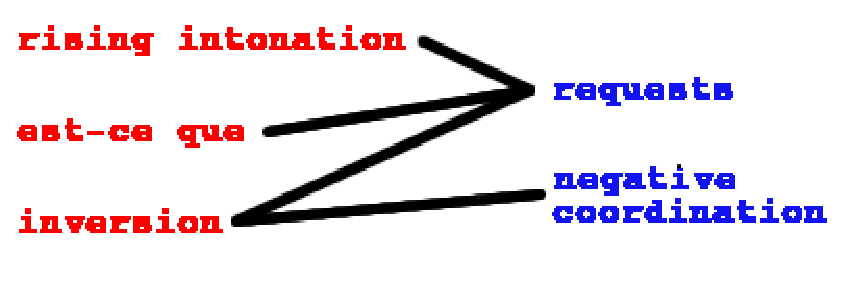
\includegraphics[width=.6\textwidth]{\imgpath/fufofomp}
\caption{Many-to-one relations of form-meaning pairs}
\label{fig:fufofomp:outro} 
\end{figure}

This relation can be expressed by a set of fo-fomps and fu-fomps as follows.\footnote{In 
 order to not complicate the example further, I dispense with the difference between universal conceptual categories like `question' and cross-linguistically common instantiations thereof, i.e. `interrogative sentence' \citep[but see][]{Lehmann1993}. This distinction is important and should be reflected in markup used for grammatical descriptions. However, in the context of this paper, it would incur too much theoretical overhead and would obscure the main line of argumentation. Future publications will explicate the relation in more detail than what can be covered here.
}

\ea\label{xml:french}
\begin{verbatim}
<fomp type="morpheme" lemma="est-ce que">
  <formaldescription>
    <prose>
      The introducer <form> est-ce que </form>  with
      the literal meaning <gloss> Is it so
      that ... ? </gloss>. In front of a following
      vowel, the form is <objectlanguage> est-ce
      qu'</objectlanguage>. Both forms are shown in
      the following examples.
    </prose>
    <examples>
      <example> [example with est-ce que]</example>
      <example> [example with est-ce qu']</example>
    </examples>
  </formaldescription>
  <functionaldescription>
    <form> Est-ce que </form> is used for <meaning>
    questions </meaning>
  </functionaldescription>
</fomp>

<fomp type="contour" lemma="H%">
  <formaldescription>
    <prose>
      The rising contour has a high tone target on the
      last syllable. 
    </prose>
    <examples>
      <example> [example with high tone target]</example>
    </examples>
  </formaldescription>
  <functionaldescription>
    This contour is used for <meaning> question
    formation </meaning>.
  </functionaldescription>
</fomp>

<fomp type="construction" lemma="Inversion">
  <formaldescription>
    <prose>
      In the <form> Inversion Construction</form>, the
      subject is repeated after the verb. Nominal subjects
      remain in front of the verb but pronominal subjects
      are deleted.
    </prose>
    <examples>
      <example> Marie danse-t-elle?</example>
      <example> (*Elle) Danse-t-elle?</example>
    </examples>
  </formaldescription>  
  <functionaldescription>  
    <prose>
      The <form> Inversion Construction</form> is used
      for <meaning> question formation </meaning> and
      for <meaning> coordination </meaning>.
    </prose>
    <examples>
      <example> Chante-t-elle? </example>
      <example> Aussi chante-t-elle bien </example>
    </examples>
  </functionaldescription>
</fomp>

<fomp type="Speechacts" lemma="Requests">
  <overview>
    <prose>
      A <meaning> request </meaning> is used to elicit
      information from the addressee.
    </prose>
  </overview>
  <instantiations>
    <prose>
      Three strategies
      can be used to form requests. These are <form>
      rising intonation </form>, <form> preposing the
      introducer <objectlanguage> est-ce
      que </objectlanguage></form>, and <form>
      inversion</form>.
    </prose>
    <examples>
      <example>  Elle danse?</example>
      <example>  Est-ce qu'elle danse danse?</example>
      <example>  Danse-t-elle?  </example>
    </examples>
    <prose>
      The first example is the least formal, the middle
      one is quite neutral, while the third one is decidedly
      formal and pertains to the written language.
    </prose>
  </instantiations>
</fomp>
\end{verbatim}
\z

This example models the many-to-many relations between form and function in a transparent way. The most relevant parts in the context of this discussion are \tag{form} \tag{/form} and \tag{meaning} \tag{/meaning}, which can be made to point to the page where the relevant formal or functional phenomenon is discussed in more detail. The reader might have noticed that the text between the tags varies and is not drawn from a restricted vocabulary. While there might be a possibility to avoid this arbitrariness in future descriptions, this is not possible when retrofitting the schema on extant descriptions. Therefore, the precise target of the form-links and the meaning-links has to be specified. So instead of

\ea \begin{verbatim}<form> preposing the introducer <objectlanguage> est-ce
que </objectlanguage></form>\end{verbatim} \z

we should have something like

\ea \begin{verbatim}<form target="est-ce que"> preposing the introducer
<objectlanguage> est-ce que </objectlanguage></form>\end{verbatim} \z

Note that the target {\tt "est-ce que"} matches the lemma tag of \texttt{<fomp type="morpheme" lemma="est-ce que">}.

In the same vein, we can rewrite 

\ea \begin{verbatim}A <meaning> request </meaning> is used to elicit
 information from the addressee.\end{verbatim}\z

as
  
\ea \begin{verbatim}A <meaning target="Requests"> request </meaning> is used
to elicit information from the addressee.\end{verbatim}\z

These targets are ideally linked to an ontology to make the references clear and consistent and facilitate cross-linguistic searches \citep{FarrarEtAl2003}. This will not be pursued here for reasons of space, but see \citet{Good2004,Goodtv} for ideas how this can be done.

\section{Interaction with the user}
As \citet{Weber2006grow} remarks, grammatical descriptions are never finished. New insights are continuously gained.\footnote{See
 \citet{Comrie1998,Cristofaro2006,Mosel2006craft,Payne2006,Rice2006} and \citet{Zaefferer2006} for similar observations.
} 
When a grammatical description is made available electronically, the findings can be updated.   \citet{Nordhoff2008jldc} discusses the  advantages of  and requirements for electronic grammar writing. An aspect not discussed in \citet{Nordhoff2008jldc} is the possibility for users to add tags to pages of an electronic description. These tags can be either arbitrary like \texttt{Compound}, \texttt{Important}, \texttt{SimilarToWarlpiri}, \texttt{Grammaticalization} or \texttt{V-Movement}. This kind of tag would have to be distinguished from a set of tags drawn from a closed restricted vocabulary. One possibility would be to rely on established schemas like the LDS questionnaire, so that tags like  \texttt{LDS\_2.3.4}  would have a clear and defined meaning. Another obvious provider for a restricted and controlled set of vocabulary would be the GOLD ontology \citep{FarrarEtAl2003}. If grammatical descriptions manage to draw a critical mass of tagging users, tag clouds can give a quick overview of the aspects of a certain page which the majority of the users find particularly relevant \citep[cf][]{BoudaEtAl2012ldl}.

\begin{figure}
 \includegraphics[width=\textwidth]{\imgpath/boxchart.png}
\caption{Visual illustration of the schema of grammatical descriptions.}
\label{fig:boxchart}
\end{figure}

\section{Schematization}
I have discussed the overall structure of a grammatical description above, including frontmatter, mainmatter and backmatter. The mainmatter was analyzed as consisting of a background part, a part for segmental phonology and two interdependent collections of form-meaning-pairs (`fomps'). The first one is based on the form-to-function or semasiological approach to grammatical analysis, while the second takes the converse onomasiological approach, function-to-form. The form-based and function-based fomps show similar structure. Both consist of alternating parts of prose and examples (Figure \ref{fig:boxchart}). These findings can be described in the RelaxNG schema given below (parts irrelevant in the context of this paper are treated as unstructured "texts" to keep the size of the schema within bounds).
\newpage
\footnotesize
\ea
\begin{verbatim}
GD =  element gd { Frontmatter,Mainmatter,Backmatter }
Frontmatter = element frontmatter { TOC, LOF, LOT, LOA, Acknowledgments }
Backmatter = element backmatter { References,Index }
Mainmatter = element mainmatter { Phonemology, Semasiology, Onomasiology }

Phonemology = element phonemology { Phonemicon }
Semasiology = element semasiology { Contouricon, Morphemicon, Constructicon }
Onomasiology = element onomasiology { Semanticon, Discoursicon, Pragmaticon }   

Phonemicon = element phonemicon  { text }
Contouricon = element contouricon  { Fo-Part }
Morphemicon = element morphemicon  { Fo-Part }
Constructicon = element constructicon  { Fo-Part }        

Semanticon = element semanticon  { Fu-Part } 
Discoursicon = element discoursicon { Fu-Part } 
Pragmaticon = element pragmaticon { Fu-Part }

Fo-Part = element fo-collection { (Fo-Collection|Fo-Fomp)* }
Fo-Collection = element fo-list { Tags,  Prose, Examples, Formlinklist }

Fu-Part = element fu-collection { (Fu-Collection|Fu-Fomp)* }
Fu-Collection = element fu-list { Tags,  Prose, Examples, Funclinklist }

Examples = element examples { Example+ }
 
Fo-Fomp = element fo-fomp { Tags,  Overview, Formaldescription, Functionaldescription }
Formaldescription = element formaldescription { (Prose|Example)* }
Functionaldescription = element functionaldescription { (Prose|Example)* }

Fu-Fomp = element fu-fomp { Tags,  Overview, Instantiations }
Instantiations = element instantiations { (Prose|Example)* }

Overview = element overview { text }
Prose = element prose { text }

Example = element example { Tags,  Bowhughesbird }
Bowhughesbird = element bowhughesbird { text }

Formlinklist = element formlinklist  { Formlink+ }
Funclinklist = element funclinklist  { Funclink+ }

Formlink = Link
Funclink = Link

Link = element link { attribute name { text }, attribute target { text } }
Tags = element tag { attribute name { text } }*

TOT = element tableofcontents { text }
LOF = element listoffigures { text }
LOT = element listoftables { text }
LOA = element listofabbreviations { text }
Acknowledgments = element acknowledgments { text }
References = element references { text }
Index = element index { text }

\end{verbatim}
\z
\normalsize

\section{Conclusion and outlook}
This paper has analyzed the semantic structure of grammatical descriptions and shown that in the domain of form-meaning pairs,  the interaction between the  semasiological and the onomasiological approach  can be formalized in a RelaxNG schema. Grammars structured along this schema have a number of advantages. First, the schema encourages encapsulation of the descriptive content. The descriptive content in each fomp should be independent of the surrounding fomps. If the schema is adhered to, the constraint of linearity disappears. The elements are self-contained, which allows for addition and modification of elements without affecting the overall structure (terminological consistency remains an issue of course). This means that grammars can be written and published in an incremental heap-like way, making new insights available to the general public as they are gained \citep[cf.][]{Weber2006grow,Goodtv}. Furthermore, the basic advantages of structured text obtain, e.g. semantic searches, extraction, modification, differential presentation \citep{Maxwelltv}.

The schema proposed here is designed to be compatible with recent structuring proposals in other domains of grammar, namely \citet{BowEtAl2003} and \citet{Good2004}. Further work in analyzing the structure of grammatical descriptions needs to be done. Issues for further theoretical work are: the structure of phonological descriptions, the nature of tags and links, and the implementation of a controlled vocabulary for certain fields through an ontology. As far as practical applications are concerned, the schema will have to be measured against the actual requirements of future and past grammars. Is it possible to use this schema when writing a grammar, and is it possible to retrofit this schema on an existing grammar? As for the former question, first results are positive. \citet{Nordhoff2009phd} is a descriptive grammar of a previously undescribed language, Sri Lanka Malay. While this grammar is not in XML-format yet, it was designed with the application of the above schema in mind. As such it contains a formal part and a functional part, which are roughly structured as outlined above. Furthermore, the individual sections in the two parts are parallel to fo-fomps and fu-fomps. The conversion process of the manuscript to XML is currently under way and looks promising. Retrofitting the schema on legacy descriptions is a more difficult task. The book has to be split into independent fomps. Depending on whether the author adhered to a strict separation of formal and functional discussion \citep[e.g.][]{Seiler1985}, the task is more or less easy. Resolving interparagraph dependencies (\em as demonstrated in the last paragraph, as shown below, contrary to what was said in the preceding section \em etc) will probably be a problematic issue in splitting the grammatical description into independent chunks on which the schema can be applied. In a first step, retrofitting will be done manually, but in a second step, semi-automatic analysis of the structure of grammatical descriptions remains a goal. Extraction tools like \citet{Lewis2006} are probably a worthwhile domain to investigate for these prospects.

The ultimate goal would be to have an online repository of all existing grammatical descriptions which are converted to XML. These could be queried in a semantic fashion. The query would yield all the descriptive content of the selected grammars about a particular domain, a very useful feature for large sample typology. While there is still a very long way to go, the GALOES platform \citep{Nordhoff2007alt,Nordhoff2007dobes,Nordhoff2007mpi} is aimed at supporting language describers in writing XML-based grammars. Descriptive departments in several European countries have expressed interest in collaboration. In the long run, this should assure that future grammatical descriptions comply with the schema. As for legacy descriptions, the next step will be an analysis of the 10,000 electronic grammars collected by Harald Hammarstöm to see how far automatic extraction procedures can get us. This topic will be treated in future papers.  

% 
% \bibliographystyle{natuva}
% \bibliography{asw,grammaticography,grammars,nordhoff}
% 
% \section{Appendix}
% \footnotesize
% \begin{verbatim}<?xml version="1.0" encoding="UTF-8"?>
% <xs:schema xmlns:xs="http://www.w3.org/2001/XMLSchema" elementFormDefault="qualified">
%   <xs:element name="gd">
%     <xs:complexType>
%       <xs:sequence>
%         <xs:element ref="frontmatter"/>
%         <xs:element ref="mainmatter"/>
%         <xs:element ref="backmatter"/>
%       </xs:sequence>
%     </xs:complexType>
%   </xs:element>
%   <xs:element name="frontmatter">
%     <xs:complexType>
%       <xs:sequence>
%         <xs:element ref="tableofcontents"/>
%         <xs:element ref="listoffigures"/>
%         <xs:element ref="listoftables"/>
%         <xs:element ref="listofabbreviations"/>
%         <xs:element ref="acknowledgments"/>
%       </xs:sequence>
%     </xs:complexType>
%   </xs:element>
%   <xs:element name="backmatter">
%     <xs:complexType>
%       <xs:sequence>
%         <xs:element ref="references"/>
%         <xs:element ref="index"/>
%       </xs:sequence>
%     </xs:complexType>
%   </xs:element>
%   <xs:element name="mainmatter">
%     <xs:complexType>
%       <xs:sequence>
%         <xs:element ref="phonemology"/>
%         <xs:element ref="semasiology"/>
%         <xs:element ref="onomasiology"/>
%       </xs:sequence>
%     </xs:complexType>
%   </xs:element>
%   <xs:element name="phonemology" type="Phonemicon"/>
%   <xs:element name="semasiology">
%     <xs:complexType>
%       <xs:sequence>
%         <xs:element ref="contouricon"/>
%         <xs:element ref="morphemicon"/>
%         <xs:element ref="constructicon"/>
%       </xs:sequence>
%     </xs:complexType>
%   </xs:element>
%   <xs:element name="onomasiology">
%     <xs:complexType>
%       <xs:sequence>
%         <xs:element ref="semanticon"/>
%         <xs:element ref="discoursicon"/>
%         <xs:element ref="pragmaticon"/>
%       </xs:sequence>
%     </xs:complexType>
%   </xs:element>
%   <xs:complexType name="Phonemicon">
%     <xs:sequence>
%       <xs:element ref="phonemicon"/>
%     </xs:sequence>
%   </xs:complexType>
%   <xs:element name="phonemicon" type="xs:string"/>
%   <xs:element name="contouricon" type="Fo-Part"/>
%   <xs:element name="morphemicon" type="Fo-Part"/>
%   <xs:element name="constructicon" type="Fo-Part"/>
%   <xs:element name="semanticon" type="Fu-Part"/>
%   <xs:element name="discoursicon" type="Fu-Part"/>
%   <xs:element name="pragmaticon" type="Fu-Part"/>
%   <xs:complexType name="Fo-Part">
%     <xs:sequence>
%       <xs:element ref="fo-collection"/>
%     </xs:sequence>
%   </xs:complexType>
%   <xs:element name="fo-collection">
%     <xs:complexType>
%       <xs:choice minOccurs="0" maxOccurs="unbounded">
%         <xs:element ref="fo-list"/>
%         <xs:element ref="fo-fomp"/>
%       </xs:choice>
%     </xs:complexType>
%   </xs:element>
%   <xs:element name="fo-list">
%     <xs:complexType>
%       <xs:sequence>
%         <xs:group ref="Tags"/>
%         <xs:element ref="prose"/>
%         <xs:element ref="examples"/>
%         <xs:element ref="formlinklist"/>
%       </xs:sequence>
%     </xs:complexType>
%   </xs:element>
%   <xs:complexType name="Fu-Part">
%     <xs:sequence>
%       <xs:element ref="fu-collection"/>
%     </xs:sequence>
%   </xs:complexType>
%   <xs:element name="fu-collection">
%     <xs:complexType>
%       <xs:choice minOccurs="0" maxOccurs="unbounded">
%         <xs:element ref="fu-list"/>
%         <xs:element ref="fu-fomp"/>
%       </xs:choice>
%     </xs:complexType>
%   </xs:element>
%   <xs:element name="fu-list">
%     <xs:complexType>
%       <xs:sequence>
%         <xs:group ref="Tags"/>
%         <xs:element ref="prose"/>
%         <xs:element ref="examples"/>
%         <xs:element ref="funclinklist"/>
%       </xs:sequence>
%     </xs:complexType>
%   </xs:element>
%   <xs:element name="examples">
%     <xs:complexType>
%       <xs:sequence>
%         <xs:element maxOccurs="unbounded" ref="example"/>
%       </xs:sequence>
%     </xs:complexType>
%   </xs:element>
%   <xs:element name="fo-fomp">
%     <xs:complexType>
%       <xs:sequence>
%         <xs:group ref="Tags"/>
%         <xs:element ref="overview"/>
%         <xs:element ref="formaldescription"/>
%         <xs:element ref="functionaldescription"/>
%       </xs:sequence>
%     </xs:complexType>
%   </xs:element>
%   <xs:element name="formaldescription">
%     <xs:complexType>
%       <xs:choice minOccurs="0" maxOccurs="unbounded">
%         <xs:element ref="prose"/>
%         <xs:element ref="example"/>
%       </xs:choice>
%     </xs:complexType>
%   </xs:element>
%   <xs:element name="functionaldescription">
%     <xs:complexType>
%       <xs:choice minOccurs="0" maxOccurs="unbounded">
%         <xs:element ref="prose"/>
%         <xs:element ref="example"/>
%       </xs:choice>
%     </xs:complexType>
%   </xs:element>
%   <xs:element name="fu-fomp">
%     <xs:complexType>
%       <xs:sequence>
%         <xs:group ref="Tags"/>
%         <xs:element ref="overview"/>
%         <xs:element ref="instantiations"/>
%       </xs:sequence>
%     </xs:complexType>
%   </xs:element>
%   <xs:element name="instantiations">
%     <xs:complexType>
%       <xs:choice minOccurs="0" maxOccurs="unbounded">
%         <xs:element ref="prose"/>
%         <xs:element ref="example"/>
%       </xs:choice>
%     </xs:complexType>
%   </xs:element>
%   <xs:element name="overview" type="xs:string"/>
%   <xs:element name="prose" type="xs:string"/>
%   <xs:element name="example">
%     <xs:complexType>
%       <xs:sequence>
%         <xs:group ref="Tags"/>
%         <xs:element ref="bowhughesbird"/>
%       </xs:sequence>
%     </xs:complexType>
%   </xs:element>
%   <xs:element name="bowhughesbird" type="xs:string"/>
%   <xs:element name="formlinklist">
%     <xs:complexType>
%       <xs:group maxOccurs="unbounded" ref="Formlink"/>
%     </xs:complexType>
%   </xs:element>
%   <xs:element name="funclinklist">
%     <xs:complexType>
%       <xs:group maxOccurs="unbounded" ref="Funclink"/>
%     </xs:complexType>
%   </xs:element>
%   <xs:group name="Formlink">
%     <xs:sequence>
%       <xs:element ref="link"/>
%     </xs:sequence>
%   </xs:group>
%   <xs:group name="Funclink">
%     <xs:sequence>
%       <xs:element ref="link"/>
%     </xs:sequence>
%   </xs:group>
%   <xs:element name="link">
%     <xs:complexType>
%       <xs:attribute name="name" use="required"/>
%       <xs:attribute name="target" use="required"/>
%     </xs:complexType>
%   </xs:element>
%   <xs:group name="Tags">
%     <xs:sequence>
%       <xs:element minOccurs="0" maxOccurs="unbounded" ref="tag"/>
%     </xs:sequence>
%   </xs:group>
%   <xs:element name="tag">
%     <xs:complexType>
%       <xs:attribute name="name" use="required"/>
%     </xs:complexType>
%   </xs:element>
%   <xs:element name="tableofcontents" type="xs:string"/>
%   <xs:element name="listoffigures" type="xs:string"/>
%   <xs:element name="listoftables" type="xs:string"/>
%   <xs:element name="listofabbreviations" type="xs:string"/>
%   <xs:element name="acknowledgments" type="xs:string"/>
%   <xs:element name="references" type="xs:string"/>
%   <xs:element name="index" type="xs:string"/>
% </xs:schema>
% 
% \end{verbatim}
% 
% \normalsize
%  
\bibliographystyle{unified}
\bibliography{asw,creole,grammars,lankahist,lgctct,malay,nordhoff,phon,tamil,grammaticography,tv}
\end{document}
